\documentclass{standalone}
\usepackage{tikz}
\usepackage{pgfplots}
\pgfplotsset{width=7cm,compat=1.8}

\begin{document}
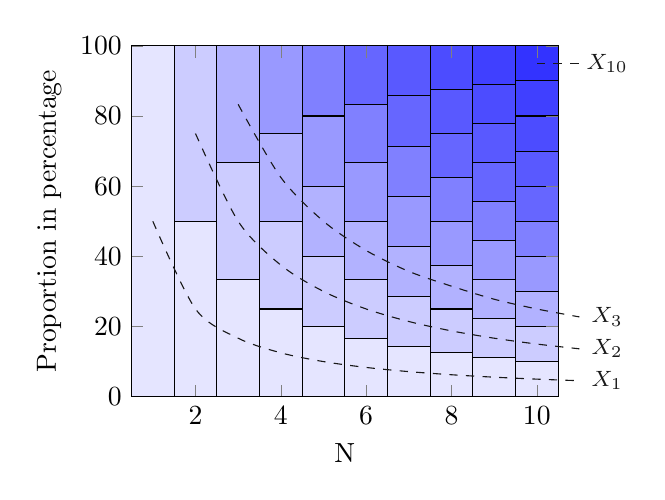
\begin{tikzpicture}
\begin{axis}[
  ybar stacked,
  bar width=1,
  axis on top,
  xmin=0.5,
  xmax=10.5,
  ymin=0,
  ymax=100,
  xlabel={N},
  ylabel={Proportion in percentage},
  after end axis/.code={
    \draw [color=black!90!white,dashed,smooth] plot coordinates{(axis cs:1,50) (axis cs:2,25) (axis cs:3,16.66666) (axis cs:4,12.5) (axis cs:5,10.0) (axis cs:6,8.33333) (axis cs:7,7.14286) (axis cs:8,6.25) (axis cs:9,5.55555) (axis cs:10,5.0) (axis cs:11,4.54545)} node [xshift=1em,font=\footnotesize] {$X_1$};
    \draw [color=black!90!white,dashed,smooth] plot coordinates{(axis cs:2,75.0) (axis cs:3,50.0) (axis cs:4,37.5) (axis cs:5,30.0) (axis cs:6,25.0) (axis cs:7,21.42857) (axis cs:8,18.75) (axis cs:9,16.66666) (axis cs:10,15.0) (axis cs:11,13.63636)} node [xshift=1em,font=\footnotesize] {$X_2$};
    \draw [color=black!90!white,dashed,smooth] plot coordinates{(axis cs:3,83.33333) (axis cs:4,62.5) (axis cs:5,50.0) (axis cs:6,41.66666) (axis cs:7,35.71486) (axis cs:8,31.5) (axis cs:9,27.77777) (axis cs:10,25.0) (axis cs:11,22.72727)} node [xshift=1em,font=\footnotesize] {$X_3$};
    \draw [color=black!90!white,dashed,smooth] plot coordinates{(axis cs:10,95.0) (axis cs:11,95.0)} node [xshift=1em,font=\footnotesize] {$X_{10}$};
  }
  ]
\addplot[fill=blue!10!white] coordinates {(1,100) (2,50.00000) (3,33.33333) (4,25.0) (5,20.0) (6,16.66666) (7,14.28571) (8,12.5) (9,11.11111) (10,10.0)};
\addplot[fill=blue!20!white] coordinates {(1,0) (2,50.00000) (3,33.33333) (4,25.0) (5,20.0) (6,16.66666) (7,14.28571) (8,12.5) (9,11.11111) (10,10.0)};
\addplot[fill=blue!30!white] coordinates {(1,0) (2,0.00000) (3,33.33333) (4,25.0) (5,20.0) (6,16.66666) (7,14.28571) (8,12.5) (9,11.11111) (10,10.0)};
\addplot[fill=blue!40!white] coordinates {(1,0) (2,0.00000) (3,0.00000) (4,25.0) (5,20.0) (6,16.66666) (7,14.28571) (8,12.5) (9,11.11111) (10,10.0)};
\addplot[fill=blue!50!white] coordinates {(1,0) (2,0.00000) (3,0.00000) (4,0.00000) (5,20.0) (6,16.66666) (7,14.28571) (8,12.5) (9,11.11111) (10,10.0)};
\addplot[fill=blue!60!white] coordinates {(1,0) (2,0.00000) (3,0.00000) (4,0.00000) (5,0.00000) (6,16.66666) (7,14.28571) (8,12.5) (9,11.11111) (10,10.0)};
\addplot[fill=blue!65!white] coordinates {(1,0) (2,0.00000) (3,0.00000) (4,0.00000) (5,0.00000) (6,0.00000) (7,14.28571) (8,12.5) (9,11.11111) (10,10.0)};
\addplot[fill=blue!70!white] coordinates {(1,0) (2,0.00000) (3,0.00000) (4,0.00000) (5,0.00000) (6,0.00000) (7,0.00000) (8,12.5) (9,11.11111) (10,10.0)};
\addplot[fill=blue!75!white] coordinates {(1,0) (2,0.00000) (3,0.00000) (4,0.00000) (5,0.00000) (6,0.00000) (7,0.00000) (8,0.00000) (9,11.11111) (10,10.0)};
\addplot[fill=blue!80!white] coordinates {(1,0) (2,0.00000) (3,0.00000) (4,0.00000) (5,0.00000) (6,0.00000) (7,0.00000) (8,0.00000) (9,0.00000) (10,10.0)};
\end{axis}

\end{tikzpicture}
\end{document}
